%-----------------------------------------------------------------
%	THEORITICAL BACKGROUND
%	!TEX root = ./../main.tex
%-----------------------------------------------------------------
\section{Theoretical Background}

%-----------------------------------------------------------------
\subsection{Knapsack Problem}
The knapsack problem is a classical 0--1 combinatorial optimization problem that can be applied to various fields such as economics. A set of $n$ items, each item $i (i = 1, \dots , n)$ has assigned a value (for instance price) $v_i$ and an item weight value $w_i$ for each item $i (i = 1, \dots , n)$. The problem is to identify a subset of all items that leads to the highest total profit and does not exceed the resource upper bound $W$ . Then, the knapsack can be formulated as:

\begin{align}\label{eq:maxf}
    \text{maximize }  f = \sum_{i=1}^{n} v_i x_i, \text{ where } x_i = 
    \begin{cases}
        1 & \text{if the item is in the bag} \\
        0 & \text{otherwise}
    \end{cases}
\end{align}

subject to the constraints
\begin{align}\label{eq:cons}
    \sum_{i=1}^{n} w_i x_i \leq W 
    \qc x_i \in \qty{0,1}
\end{align}

The variable $x_i$ is an indicator of item $i$. If $x_i$ is set to \num{1}, it means item $i$ is selected, or \num{0} means item $i$ is not selected for $i = 1, \dots , n$. \eqref{eq:maxf} represents the total value or profit of selection items and \eqref{eq:cons} constraint.

%-----------------------------------------------------------------
\subsection{Simulated Annealing}\label{sec:sa}
Simulated annealing is so named because of its analogy to the process of physical annealing with solids, in which a crystalline solid is heated and then allowed to cool very slowly until it achieves its most regular possible crystal lattice configuration (i.e., its minimum lattice energy state), and thus is free of crystal defects. If the cooling schedule is sufficiently slow, the final configuration results in a solid with such superior structural integrity. Simulated annealing establishes the connection between this type of thermodynamic behavior and the search for global minimum for a discrete optimization problem. Furthermore, it provides an algorithmic means for exploiting such a connection.

At each iteration of a simulated annealing algorithm applied to a discrete optimization problem, the objective function generates values for two solutions (the current solution and a newly selected solution) are compared. Improving solutions are always accepted, while a fraction of non-improving (inferior) solutions are accepted in the hope of escaping local optima in search of global optima. The probability of accepting non-improving solutions depends on a temperature parameter, which is typically non-increasing with each iteration of the algorithm.

\subsubsection*{Steps of the Algorithm}
The usual steps for Simulated Annealing are presented below:
\begin{enumerate}[(i)]
    \item \emph{Initialize}: start with a random initial placement. Initialize a very high “temperature”.
    \item \emph{Move}: perturb the placement through a defined move.\label{step2}
    \item \emph{Calculate Score}: Calculate the change in the score due to the move made. 
    \item \emph{Choose}: depending on the change in score, accept or reject the move, where probability of acceptance depends on the current “temperature”. For this point we will use the Classical Metropolis Method.
    \item \emph{Update and Repeat}: update the temperature value by
    lowering the temperature following a cooling schedule. Go back to \ref{step2}.
\end{enumerate}

The process is done when the “Freezing Point” is reached.

\subsubsection*{Acceptance Rule}
In thermodynamical systems, it is usual to use the Classical Metropolis Method to compute the probability of changing from one state to another~\cite{Frenkel2002}. In simple words, the method consists on doing a random change in the system and accept the change in accordance to the following acceptance rule:
\begin{align}
	\acc{\va{x}}{\va{y}} =
	\begin{cases}
		e^{- \beta \qty[H(\va{y}) - H(\va{x})]} & H(\va{y}) > H(\va{x}) \\
		1                                       & H(\va{y}) < H(\va{x})
	\end{cases}
\end{align}
where $H(\va{x})$ is the energy of the state $\va{x}$, $\beta = 1/(k_{B} T)$, and $T$ is the temperature.

Notice that this has the same physical interpretation we would expect in a thermodynamical system:
\begin{itemize}
	\item Limit $T \to 0$ ($\beta \to \infty$): the system only accepts changes that minimize the energy:
	\begin{align*}
		\acc{\va{x}}{\va{y}} =
		\begin{cases}
			0 & H(\va{y}) > H(\va{x}) \\
			1 & H(\va{y}) < H(\va{x})
		\end{cases}
	\end{align*}
	\item Límit $T \to \infty$ ($\beta \to 0$): the system accepts all changes, which maximizes the entropy.
\end{itemize}

In our problem, the \emph{energy} can be interpreted as follows:
\begin{align}
    H(\va{x}) = \displaystyle \sum_{i=1}^{n} v_i x_i
\end{align}

\subsubsection*{Cooling Schedule}
In the process of annealing a metal, if the heating temperature is sufficiently high to ensure random state and the cooling process is slow enough to ensure thermal equilibrium, then the atoms will place themselves in a pattern that corresponds to the global energy minimum of a perfect crystal.

For this reason, we need to choose very carefully our Cooling Schedule. We have decided to use a curve that decreases slowly the temperature until the particles arrange themselves in the ground state of the solid. We use the following formula:
\begin{align}
    T_{i} = \frac{T_{0} \cdot \tanh(- \ln(i) + 10) + 1 )}{2} 
\end{align}

The idea behind it is to let the algorithm quickly discard bad configurations in the very beginning (high temperature), and explore different configurations close to the optimal solution in the final steps (low temperatures). The plot of the our cooling schedule can be seen in \cref{fig:temp}.
\begin{figure}[H]
    \centering
    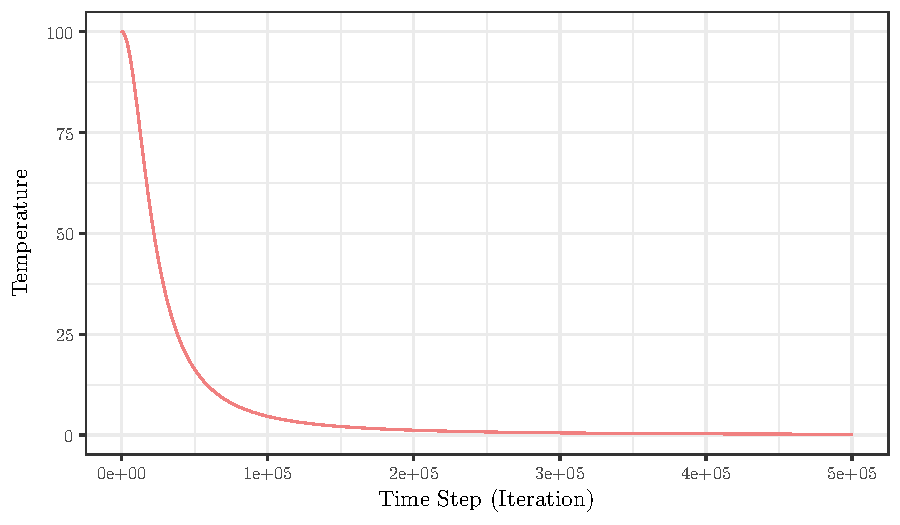
\includegraphics[width=\textwidth]{images/temp}
    \caption{Evolution of the Temperature Following a Cooling Schedule}
    \label{fig:temp}
\end{figure}









